
\renewcommand{\thesection}{\Alph{section}}
\renewcommand{\thefigure}{A\arabic{figure}}
\renewcommand{\tablename}{Tabla}
\renewcommand{\thetable}{A\arabic{table}}

\section{Instrucciones de armado} \label{apendice:instrucciones_armado}

\subsection{Renovación del Horiba PTI Quanta Master 400} \label{subsec:refur-instructions}

El proceso de ensamblaje para la renovación del espectrómetro Horiba PTI Quanta Master 400 se puede organizar en cinco pasos: (1) conectar el motor de excitación $M_1$ (\textbf{Fig. \ref{fig:hardware}}), (2) conectar el fin de carrera de excitación, (3) conectar el motor de emisión $M_2$, (4) conectar el fin de carrera de excitación y (5) conectar la salida del PMT. 
Las fuentes de alimentación deben permanecer apagadas hasta que todo esté correctamente conectado, como se muestra en el esquema (\textbf{Fig. \ref{fig:schematic}}). 
Es necesario asegurarse de que el voltaje de GND sea el mismo en todas las conexiones. 
\textbf{Advertencia:} configurar límite de corriente del controlador DRV8825 esté configurado correctamente (en nuestro caso, para limitar a 0.7 A) y que los pines estén conectados adecuadamente, de lo contrario existe el riesgo de que circule demasiada corriente por los bobinados de los motores y se dañen.

\begin{enumerate}
    \item \textbf{Conectar el motor de excitación}
    \begin{enumerate}
        \item Conectar los pines P6 y P7 del RP a los pines STEP y DIR del DRV8825, respectivamente (\textbf{Fig. \ref{fig:schematic}}).
        \item Conectar los pines restantes: utilizando 3.3 V del RP como nivel alto digital, coloque los pines $\overline{\text{SLEEP}}$ y $\overline{\text{RESET}}$ del controlador del motor en alto, y conecte el GND lógico al GND del RP. Los pines $\overline{\text{ENABLE}}$, M0, M1, M2 y $\overline{\text{FAULT}}$ pueden dejarse flotantes.
        \item Ajustar el límite de corriente de salida del DRV8825 al máximo soportado por el motor paso a paso; en este caso, el motor M061CS02 tiene un límite de 0.7 A.
        \item Provea la fuente de alimentación del motor conectando los pines VMOT y GND a una fuente de 12 V que pueda suministrar al menos $2 \times \textit{límite de corriente}$. Conectar un capacitor de 100 $\mu F$ en paralelo.
        \item Conectar el controlador del motor al motor paso a paso: desconecte el conector original del motor $M_1$ y conecte los pines A1 y A2 del DRV8825 a los pines 1 y 7 del motor, y los pines B1 y B2 a los pines 3 y 5 (\textbf{Fig. \ref{fig:hardware}B}).
    \end{enumerate}
    \item \textbf{Conectar el fin de carrera de excitación}
    \begin{enumerate}
        \item Alimentar con 5 V y GND a los pines 1 y 2, respectivamente, del fin de carrera junto al motor $M_1$ (\textbf{Fig. \ref{fig:hardware}C}).
        \item Conectar el pin 3 del fin de carrera al pin digital P2 del RP para el fin de carrera de $M_1$, utilizando una resistencia pull-up externa al nivel lógico de 3.3 V del RP.
    \end{enumerate}
    \item \textbf{Conectar el motor de emisión}
    \begin{enumerate}
        \item Conectar los pines P4 y P5 del RP a los pines STEP y DIR del controlador del motor, respectivamente.
        \item Repetir los pasos (b) a (e) del ítem (1) para el motor $M_2$.
    \end{enumerate}
    \item \textbf{Conectar el fin de carrera de emisión}
    \begin{enumerate}
        \item Alimentar con 5 V y GND a los pines 1 y 2, respectivamente, del fin de carrera junto al motor $M_2$ (\textbf{Fig. \ref{fig:hardware}C}).
        \item Conectar el pin 3 del fin de carrera al pin digital P3 del RP para el fin de carrera de $M_2$, utilizando una resistencia pull-up externa al nivel lógico de 3.3 V del RP.
    \end{enumerate}
    \item \textbf{Conectar la salida del PMT}
    \begin{enumerate}
        \item Conectar el cable BNC-SMA a la entrada analógica 1 del RP y configurar el modo de alto voltaje.
        \item Conectar una ficha T BNC al extremo BNC del cable BNC-SMA conectado al RP.
        \item Conectar una terminación de 50 $\Omega$ a uno de los extremos de la ficha T para conformar pulsos de 40 a 100 ns.
        \item Conectar el otro extremo de la ficha T a la salida del PMT utilizando un cable BNC-BNC.
    \end{enumerate}
\end{enumerate}

\noindent Después de estos pasos, el instrumento estará listo para realizar mediciones estacionarias.

\begin{SCfigure}[][h]
         \centering
         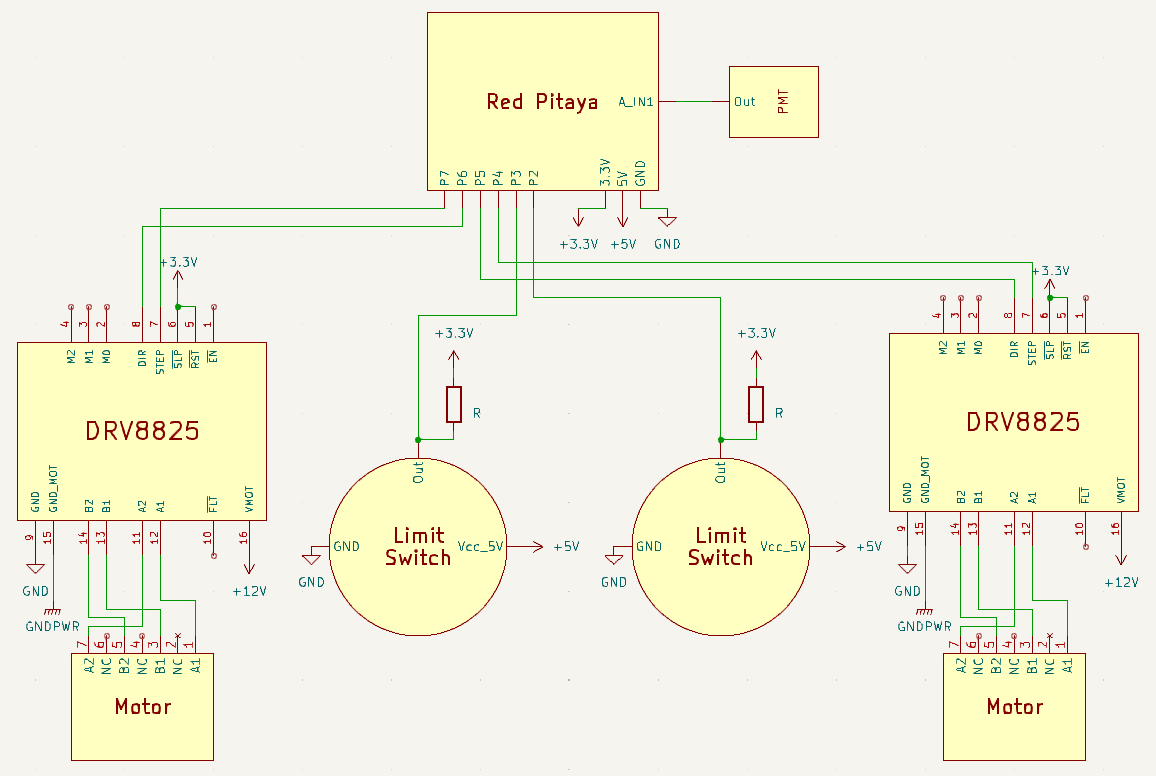
\includegraphics[width=.65\textwidth]{schematic.png}
         \caption{\textbf{Esquemático de las conexiones} que contiene la placa PCB de prueba para conectar las componentes del hardware a la RP.
         }
         \label{fig:schematic}
    \end{SCfigure}


\subsection{Ampliación para mediciones dinámicas}

Para añadir la funcionalidad de medir tiempos de vida con el espectrómetro Horiba PTI, además de las instrucciones anteriores, deben realizarse los siguientes pasos adicionales:

\begin{enumerate}
    \item Conectar la fuente de luz externa al puerto externo utilizando un cable de fibra óptica.
    \item Conectar el puerto USB tipo B del ITC4020 al puerto USB tipo A del RP.
    \item Conectar la salida BNC R3 (salida TTL de 5 V del ITC4020) en el panel trasero del ITC4020 a un adaptador BNC a SMA, y luego conectarlo a la entrada analógica 2 del RP configurando ese canal en modo de alto voltaje.
\end{enumerate}

Nuestro software está diseñado para trabajar con el controlador láser ITC4020, pero se puede utilizar otro siempre y cuando se añadan clases de control específicas al software.

\subsection{Instalación y configuración del software} \label{apendice:instalacion}

Seguir las instrucciones en \href{https://github.com/tdinapoli/refurbishedPTI}{este enlace}\cite{napoli_tdinapoli_2024} para instalar nuestro paquete Python en su RP. 
Una vez conectados los componentes de hardware, se deben calibrar los motores de los monocromadores y las entradas analógicas de la Red Pitaya. 
Las instrucciones para calibrar las entradas analógicas del RP están disponibles en su documentación oficial \cite{rp_docs}.

Para calibrar los monocromadores, desarrollamos un intérprete de línea de comandos que guía el proceso paso a paso y genera un archivo YAML con los parámetros de calibración (\textbf{Tabla \ref{tab:monochromator_api_parameters}}). El siguiente código en Python abre el menú para calibrar el monocromador de emisión:

\begin{lstlisting}[language=Python]
from refurbishedPTI import Spectrometer
spec = Spectrometer.constructor_default()
spec.emission_mono.calibrate()
\end{lstlisting}

El comando \texttt{save\_to\_yaml} guarda el archivo de configuración en el directorio del RP indicado por el método \texttt{.get\_config\_path()} de la clase Motor. Una vez calibrado el monocromador de emisión, repita el proceso para el monocromador de excitación:

\begin{lstlisting}[language=Python]
spec.excitation_mono.calibrate()
\end{lstlisting}

Repetir los mismos pasos que para el monocromador de emisión para completar la configuración.

\begin{table}[h]
 \centering
 \begin{tabular}{|l|l|p{10cm}|}
    \hline
    \textbf{Parámetro} & \textbf{Tipo de dato} & \textbf{Descripción} \\ \hline
    \texttt{greater\_wl\_cw}          & bool               & True si la longitud de onda incrementa al girar en sentido horario, Falso en el caso contrario. \\ \hline
    \texttt{max\_wl}                 & float              & Longitud de onda máxima (en nanómetros) que permitirá configurar la API del monocromador \\ \hline
    \texttt{min\_wl}                 & float              & Longitud de onda mínima (en nanómetros) que permitirá configurar la API del monocromador \\ \hline
    \texttt{wl\_step\_ratio}          & float              & Cambio (en nanómetros) de longitud de onda por cada paso que da el motor.\\ \hline
    \texttt{home\_wavelength}        & float              & Longitud de onda (en nanómetros) en la que se activa la señal del fin de carrera. \\ \hline
\end{tabular}
\caption{\textbf{Parámetros de la API de la clase Monochromator.}}
\label{tab:monochromator_api_parameters}
\end{table}

\section{Instrucciones de uso} \label{apendice:instrucciones_uso}

Como se comentó en la sección \ref{sec:software}, hay dos formas de operar el espectrómetro renovado: a través de la API de Python y mediante la interfaz gráfica Jupyter Notebook con IPython Widgets. 

Para ambos modos de operación, todos los instrumentos listados en la explicación de la sección \ref{subsec:refur-instructions} deben estar conectados, y tanto el PMT como la lámpara deben estar encendidos. 
Se deben ajustar las rendijas de Em y Ex (\textbf{Fig. \ref{fig:ref-diagram}}) según las necesidades del experimento. 
Una vez completados estos pasos, se puede proceder con las siguientes secciones para el modo de operación por script o GUI.

\subsection{Modo de operación GUI}

La interfaz gráfica del espectrómetro se encuentra en un Jupyter Notebook que permite al usuario cambiar los parámetros del instrumento mediante Widgets de Jupyter.  
La GUI se compone de dos secciones: el panel de parámetros y el panel de gráficos (\textbf{Figs. \ref{fig:spectrum_gui}} y \textbf{\ref{fig:lifetime_gui}}).  
El panel de parámetros contiene menús desplegables, botones y campos de texto para especificar los parámetros de medición y del archivo de medición.  
El panel de gráficos incluye dos gráficos, uno para mediciones de espectro y otro para mediciones de tiempo de vida.  

Para inicializar el modo GUI del QM400 renovado, se debe abrir el notebook \texttt{gui.ipynb} ubicado en \texttt{/home/jupyter/refurbishedPTI/gui.ipynb}.  
Al ejecutar la primera celda del notebook con el código:

\begin{lstlisting}[language=Python]
from refurbishedPTI.gui import Gui
gui = Gui()
\end{lstlisting}

\noindent se inicializa la GUI. 

Para realizar una medición seleccionar las opciones \textbf{Spectrum} o \textbf{Lifetime} en el menú desplegable \textbf{Measurement type}.  
Se especifican los parámetros de la medición utilizando los componentes de la GUI (detallados en las \textbf{Tablas \ref{tab:spectrum_measurement}} y \textbf{\ref{tab:lifetime_measurement}}) y comenzar la adquisición.  
Una vez finalizada la medición, guarde y manipule los datos con los componentes de la GUI (\textbf{Tabla \ref{tab:file_parameters}}).

\begin{table}
    \centering
    \begin{tabularx}{\textwidth}{|l|X|}
        \hline
        \textbf{Parámetro} & \textbf{Descripción} \\
        \hline
        \multirow{3}{3cm}{Spectrum type} & \textbf{Emission}: monocromador de excitación fijo y monocromador de emisión se mueve. \\
        \cline{2-2}
        & \textbf{Excitation}: monocromador de emisión fijo y monocromador de excitación se mueve. \\
        \cline{2-2}
        & \textbf{Laser}: monocromador de emisión se mueve y se usa el láser externo para excitar. \\
        \hline
        Static monochromator wavelength & Longitud de onda del monocromador fijo (nm). \\
        \hline
        Starting wavelength & Longitud de onda inicial del rango escaneado (nm). \\
        \hline
        Ending wavelength & Longitud de onda final del rango escaneado (nm). \\
        \hline
        Wavelength step & Diferencia en longitud de onda entre cada dato(nm). \\
        \hline
        Acquire & Comienza la medición. \\
        \hline
    \end{tabularx}
    \caption{\textbf{Parámetros de configuración de una medición de espectro estático}.}
    \label{tab:spectrum_measurement}
\end{table}

\begin{table}[htbp]
    \centering
    \begin{tabularx}{\textwidth}{|l|X|}
        \hline
        \textbf{Parámetro} & \textbf{Descripción} \\
        \hline
        Pump power & Potencia de excitación del láser (mW). \\
        \hline
        Frequency & Frecuencia de encendido y apagado del láser. \\
        \hline
        Duty Cycle & Ciclo de trabajo del láser en \%. \\
        \hline
        Emission monochromator wavelength & Longitud de onda para la cual se medirá el tiempo de vida (nm). \\
        \hline 
        Amount of counts & Cantidad de cuentas a medir antes de terminar la medición. \\
        \hline
        Starting time & Tiempo después del \textit{trigger} hasta empezar a contar (ms). \\
        \hline
        Ending time & Tiempo después del \textit{trigger} antes de parar de contar (ms). \\
        \hline
        Acquire & Comienza la adquisición.\\
        \hline
    \end{tabularx}
    \caption{\textbf{Parámetros de configuración de una medición dinámica}.}
    \label{tab:lifetime_measurement}
\end{table}

\begin{table}[htbp]
    \centering
    \begin{tabularx}{\textwidth}{|l|X|}
        \hline
        \textbf{Parámetro} & \textbf{Descripción} \\
        \hline
        Measurement filename & Seleccione un nombre de archivo y un directorio donde se guardará la medición una vez que se presione el botón \textbf{Save}. Si no se selecciona un nombre de archivo al momento de presionar el botón \textbf{Acquire}, el nombre de archivo será la fecha y hora actuales. \\
        \hline
        Selected measurement & Seleccionar una medición para guardarla o eliminarla. \\
        \hline
        Save & Guardar una medición con el nombre, directorio y formato seleccionado. \\
        \hline
        Delete & Eliminar la medición seleccionada. \\
        \hline
        \multirow{3}{3cm}{Save to} & Formato del arcihvo en el que se guardarán los datos. Opciones: \\
        \cline{2-2}
        & \textbf{pickle} \\
        \cline{2-2}
        & \textbf{csv} \\
        \cline{2-2}
        & \textbf{excel} \\
        \hline
    \end{tabularx}
    \caption{\textbf{Parámetros de configuración del archivo que guarda los datos de una medición}.}
    \label{tab:file_parameters}
\end{table}

\begin{figure}
    \centering
    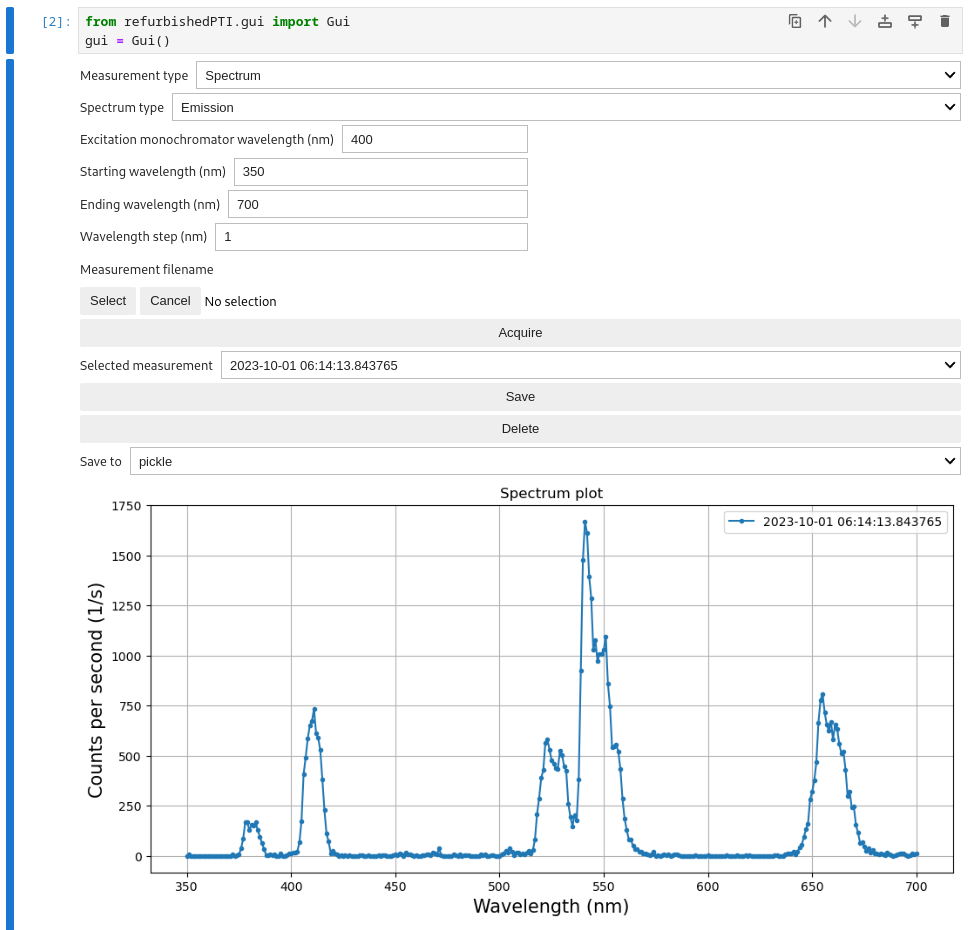
\includegraphics[width=\textwidth]{spectrum_gui.png}
    \caption{\textbf{GUI para medir espectros estacionarios}.}
    \label{fig:spectrum_gui}
\end{figure}

\begin{figure}
    \centering
    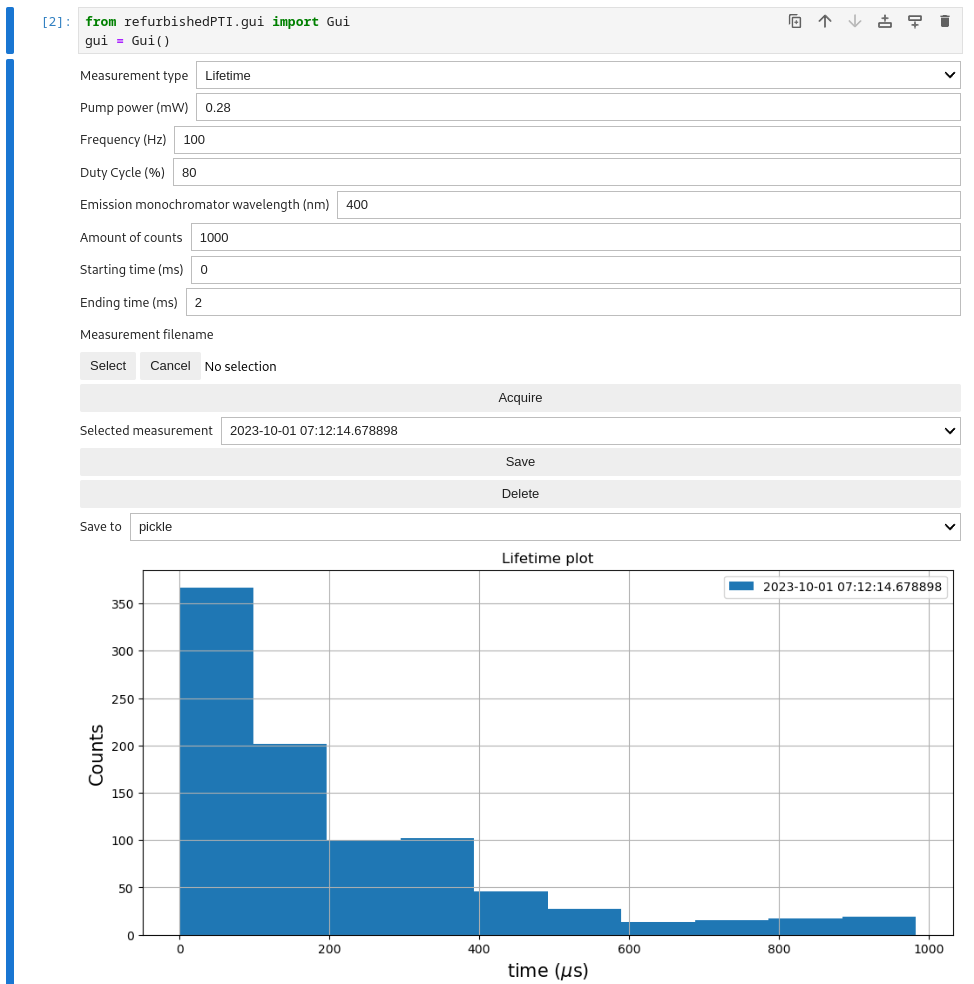
\includegraphics[width=\textwidth]{lifetime_gui.png}
    \caption{\textbf{GUI para medir tiempos de vida}.}
    \label{fig:lifetime_gui}
\end{figure}

\subsection{Modo de operación con la API de Python}

\subsubsection{Medición de espectro estacionario} \label{sec:spec_mes}

El software que desarrollamos permite al usuario realizar mediciones tanto de espectros de emisión como de excitación. En ambos casos, el primer paso es inicializar el espectrómetro:

\begin{lstlisting}[language=Python]
from refurbishedPTI.instruments import Spectrometer
spec = Spectrometer.constructor_default()
\end{lstlisting}

\noindent El método \texttt{constructor\_default()} inicializa el espectrómetro configurando los monocromadores de emisión y excitación mediante la clase Monochromator del módulo instruments.py, junto con un objeto Oscilloscope de \textit{redpipy}.
Ambas instancias de Monochromator se configuran con los archivos \texttt{emission\_init.yaml} y \texttt{excitation\_init.yaml}, que se guardan en la ruta de directorio devuelta por el método \texttt{.get\_config\_path()} de Monochromator.
Estos archivos especifican los pines de la Red Pitaya utilizados para cada controlador de motor y la ruta del archivo de calibración del monocromador.
De manera alternativa, el usuario puede inicializar diferentes instancias de monocromadores de excitación y emisión, así como del osciloscopio, y pasarlas a la clase Spectrometer para inicializarla.

Una vez inicializado el espectrómetro, ambos monocromadores deben ser llevados a su posición incial, es decir, deben moverse a la longitud de onda que activa el fin de carrera. Esto puede hacerse con el comando:

\begin{lstlisting}[language=Python]
spec.home()
\end{lstlisting}

\noindent Alternativamente, se puede establecer la longitud de onda actual de cada monocromador con:

\begin{lstlisting}[language=Python]
spec.excitation_mono.set_wavelength(ex_wl)
spec.emission_mono.set_wavelength(em_wl)
\end{lstlisting}

\noindent donde \texttt{ex\_wl} y \texttt{em\_wl} son variables que contienen los valores de las longitudes de onda actuales de cada monocromador. 
Finalmente, para obtener el espectro de emisión se usa:

\begin{lstlisting}[language=Python]
df = spec.get_emission(
    integration_time=0.01,     # En segundos
    excitation_wavelength=400, # En nanómetros
    starting_wavelength=500,   # En nanómetros
    ending_wavelength=700,     # En nanómetros
    wavelength_step=1          # En nanómetros
)
\end{lstlisting}

\noindent donde \texttt{integration\_time} es el tiempo de integración de cada punto de datos, \texttt{excitation\_wavelength} es la longitud de onda en la que se configurará el monocromador de la lámpara, y \texttt{starting\_wavelength}, \texttt{ending\_wavelength} y \texttt{wavelength\_step} son la longitud de onda inicial, final y el intervalo entre puntos de datos del espectro, respectivamente. Este método devuelve un \texttt{DataFrame} de Pandas con columnas para longitud de onda, cuentas de fotones por segundo y tiempo de integración. El \texttt{DataFrame} también contiene valores en \texttt{attrs} que especifican el tipo de espectro (emisión, excitación o láser) y la longitud de onda del monocromador estático durante el experimento. 

El proceso para obtener un espectro de excitación es análogo, pero se usa el método \texttt{get\_excitation}, cuyos argumentos son los mismos que los de \texttt{get\_emission}, excepto \texttt{excitation\_wavelength}, que se reemplaza por \texttt{emission\_wavelength}.

\subsubsection{Medición de tiempos de vida}

Para realizar una medición de tiempo de vida, es necesario configurar tanto la fuente de alimentación del diodo láser como el espectrómetro. Para controlar el diodo láser, se debe inicializar el controlador ITC4020:

\begin{lstlisting}[language=Python]
from refurbishedPTI.instruments import ITC4020
itc = ITC4020()
\end{lstlisting}

\noindent Con el controlador del láser inicializado, se pueden establecer sus parámetros mediante la API de ITC. Estos parámetros son un subconjunto de los especificados en el manual del instrumento. En este ejemplo, solo se configuran los parámetros relevantes para el experimento de tiempo de vida: el ciclo de trabajo (\textit{duty cycle}), la corriente del láser y la frecuencia. Antes de configurarlos, el ITC debe estar en modo de onda cuasi-continua (\textit{Quasi-Continuous Wave, QCW}). Los comandos correspondientes son:

\begin{lstlisting}[language=Python]
itc.qcw_mode = True
itc.frequency(100) # Frecuencia: 100 Hz
itc.current(0.1)   # Corriente: 0.1 A
itc.duty_cycle(80) # Ciclo de trabajo: 80%
\end{lstlisting}

Una vez configurados estos parámetros, el láser puede encenderse con:

\begin{lstlisting}[language=Python]
itc.laser_on(True)
\end{lstlisting}

\noindent Finalmente, con el objeto \texttt{Spectrometer} inicializado como se describe en la sección \ref{sec:spec_mes}, configure el espectrómetro y adquiera el tiempo de llegada de los fotones con:

\begin{lstlisting}[language=Python]
spec.set_decay_configuration()
counts = spec.acquire_decay(
    t0=0,               # En ms después del disparo
    tf=2,               # En ms después del disparo
    amount_counts=1000, # Número de cuentas
)
\end{lstlisting}

\noindent donde \texttt{t0} es el tiempo entre el disparo y el inicio de la adquisición, \texttt{tf} es el tiempo entre el disparo y el final de la adquisición, y \texttt{amount\_counts} es la cantidad de cuentas hasta que se detiene la adquisición. Este método devuelve un \texttt{DataFrame} de Pandas con una columna llamada \texttt{arrival\_times} que contiene los tiempos de llegada de los fotones.


